% =============================================================================
%  PIDS - Proyecto 2: Sistema de detección de vehículos y conducción autónoma
%  Bloque 3: Integración y despliegue de la red neuronal en el RoboMaster
%
%  Compilar desde este directorio (guides/PIDS):
%      pdflatex guide3.tex   (dos veces, para resolver las referencias)
% =============================================================================
\documentclass[12pt,a4paper]{article}

\usepackage[utf8]{inputenc}
\usepackage[a4paper, total={7in, 9.75in}, bottom=1in]{geometry}
\usepackage{graphicx}
\usepackage{caption}
\usepackage{subcaption}
\usepackage{framed}
\usepackage{hyperref}

% Rótulos en español (el documento lo está)
\renewcommand{\figurename}{Figura}
\renewcommand{\tablename}{Tabla}

\graphicspath{{./}{../}}

% ---------------- HEADER ----------------
\usepackage{fancyhdr}
\usepackage{graphicx}
\usepackage{xcolor}
\setlength{\headsep}{35pt}

\pagestyle{fancy}
\fancyhf{}

% Line
\renewcommand{\headrulewidth}{0.4pt}
\renewcommand{\headrule}{
\hbox to\headwidth{
  \color{gray}\leaders\hrule height \headrulewidth\hfill}
}

% Center (left header)
\fancyhead[L]{
    \begin{minipage}{10cm}
        \scriptsize \textbf{Proyectos en Ingeniería de Datos y Sistemas (PIDS)}\\
        \scriptsize Proyecto 2: Sistema de detección de vehículos y conducción autónoma
    \end{minipage}
}

% Right: group/university + logo aligned horizontally
\fancyhead[R]{
    \begin{minipage}{5.2cm}
        \scriptsize \textbf{Universidad Politécnica de Madrid}\\
        \scriptsize Grupo de Tratamiento de Imágenes
    \end{minipage}
    \raisebox{-0.3\height}{
        
\includegraphics[height=0.8cm]{header/logo_upm.pdf}
    }
}


\begin{document}

% =============================================================================
%  Título
% =============================================================================
\begin{center}
    \vspace*{.15cm}
    {\Huge \bfseries Bloque 3: Integración y despliegue de la red neuronal en el RoboMaster} \\[0.5cm]
\end{center}


% =============================================================================
\section{Introducción}
\label{sec:semana3-intro}
% =============================================================================

En este último bloque llevaremos a cabo la \underline{\textbf{integración en hardware}} del detector entrenado en el Bloque 2. En un proyecto real, integrar implica seleccionar y montar el hardware, adaptar la red a sus limitaciones, optimizar la inferencia en tiempo real, evaluar en entorno controlado y, por último, probar en el mundo real. Aquí nos quedaremos en la integración y la evaluación en un entorno controlado.

Para ello usaremos la \underline{\textbf{SDK de Python}} del RoboMaster, que permite controlar el robot desde el ordenador. Con ella diseñaremos un circuito en el que nuestro robot deberá recorrer un trayecto, buscar RoboMasters adversarios, detectarlos con nuestra red y dispararles para dejarlos fuera de combate. Esto supone decidir cómo se mueve el robot, cómo gira su torreta, cuándo ejecuta la detección y cómo dispara a lo que encuentra. Además, cada grupo podrá añadir funcionalidades propias (luces, sonidos, recorridos más elaborados, etc.) para enriquecer la demo final.


% =============================================================================
\section{VSCode}
\label{sec:semana3-vscode}
% =============================================================================

Como no es posible conectarse a los RoboMasters desde JupyterHub, esta parte la desarrollaremos en VSCode. Abra la aplicación y cargue el proyecto de la carpeta \textit{/home/PIDS/robomaster} (figura~\ref{fig:semana3-vscode-dir}). Encontrará \textit{connect.py} para conectar el robot, \textit{demo.py} para programar la demo, y varios scripts de ejemplo con los que aprender a manejar cada módulo.

Antes de ejecutar nada, asegúrese de que el intérprete seleccionado es el entorno virtual preparado para la práctica (Python 3.8). Aparece en la esquina inferior derecha (figura~\ref{fig:semana3-vscode-venv}). Si no es el correcto, haga click sobre él o pulse Ctrl+Shift+P y escriba ``Select Interpreter''. La ruta es \textit{/home/PIDS/robomaster/.pixi/venv/bin/python}.

Para ejecutar un script, ábralo y pulse Ctrl+F5 seleccionando ``Python Debugger'', o despliegue el menú junto al botón ``Play'' de la esquina superior derecha y elija ``Run Python File'' (la primera vez). A partir de ahí bastará con pulsar el botón ``Play'' para volver a lanzar el mismo script. Para depurar código, haga click a la izquierda del número de línea donde quiera detenerse; aparecerá un círculo rojo (un \textit{breakpoint}). Al lanzar el script con ``Python Debugger'', la ejecución se parará ahí y podrá inspeccionar el valor de las variables y avanzar paso a paso con los botones de la barra de depuración. Para detener una ejecución, pulse Shift+F5 o Ctrl+C.


\begin{figure}[t]
\centering
    \begin{subfigure}{0.85\textwidth}
        \centering
        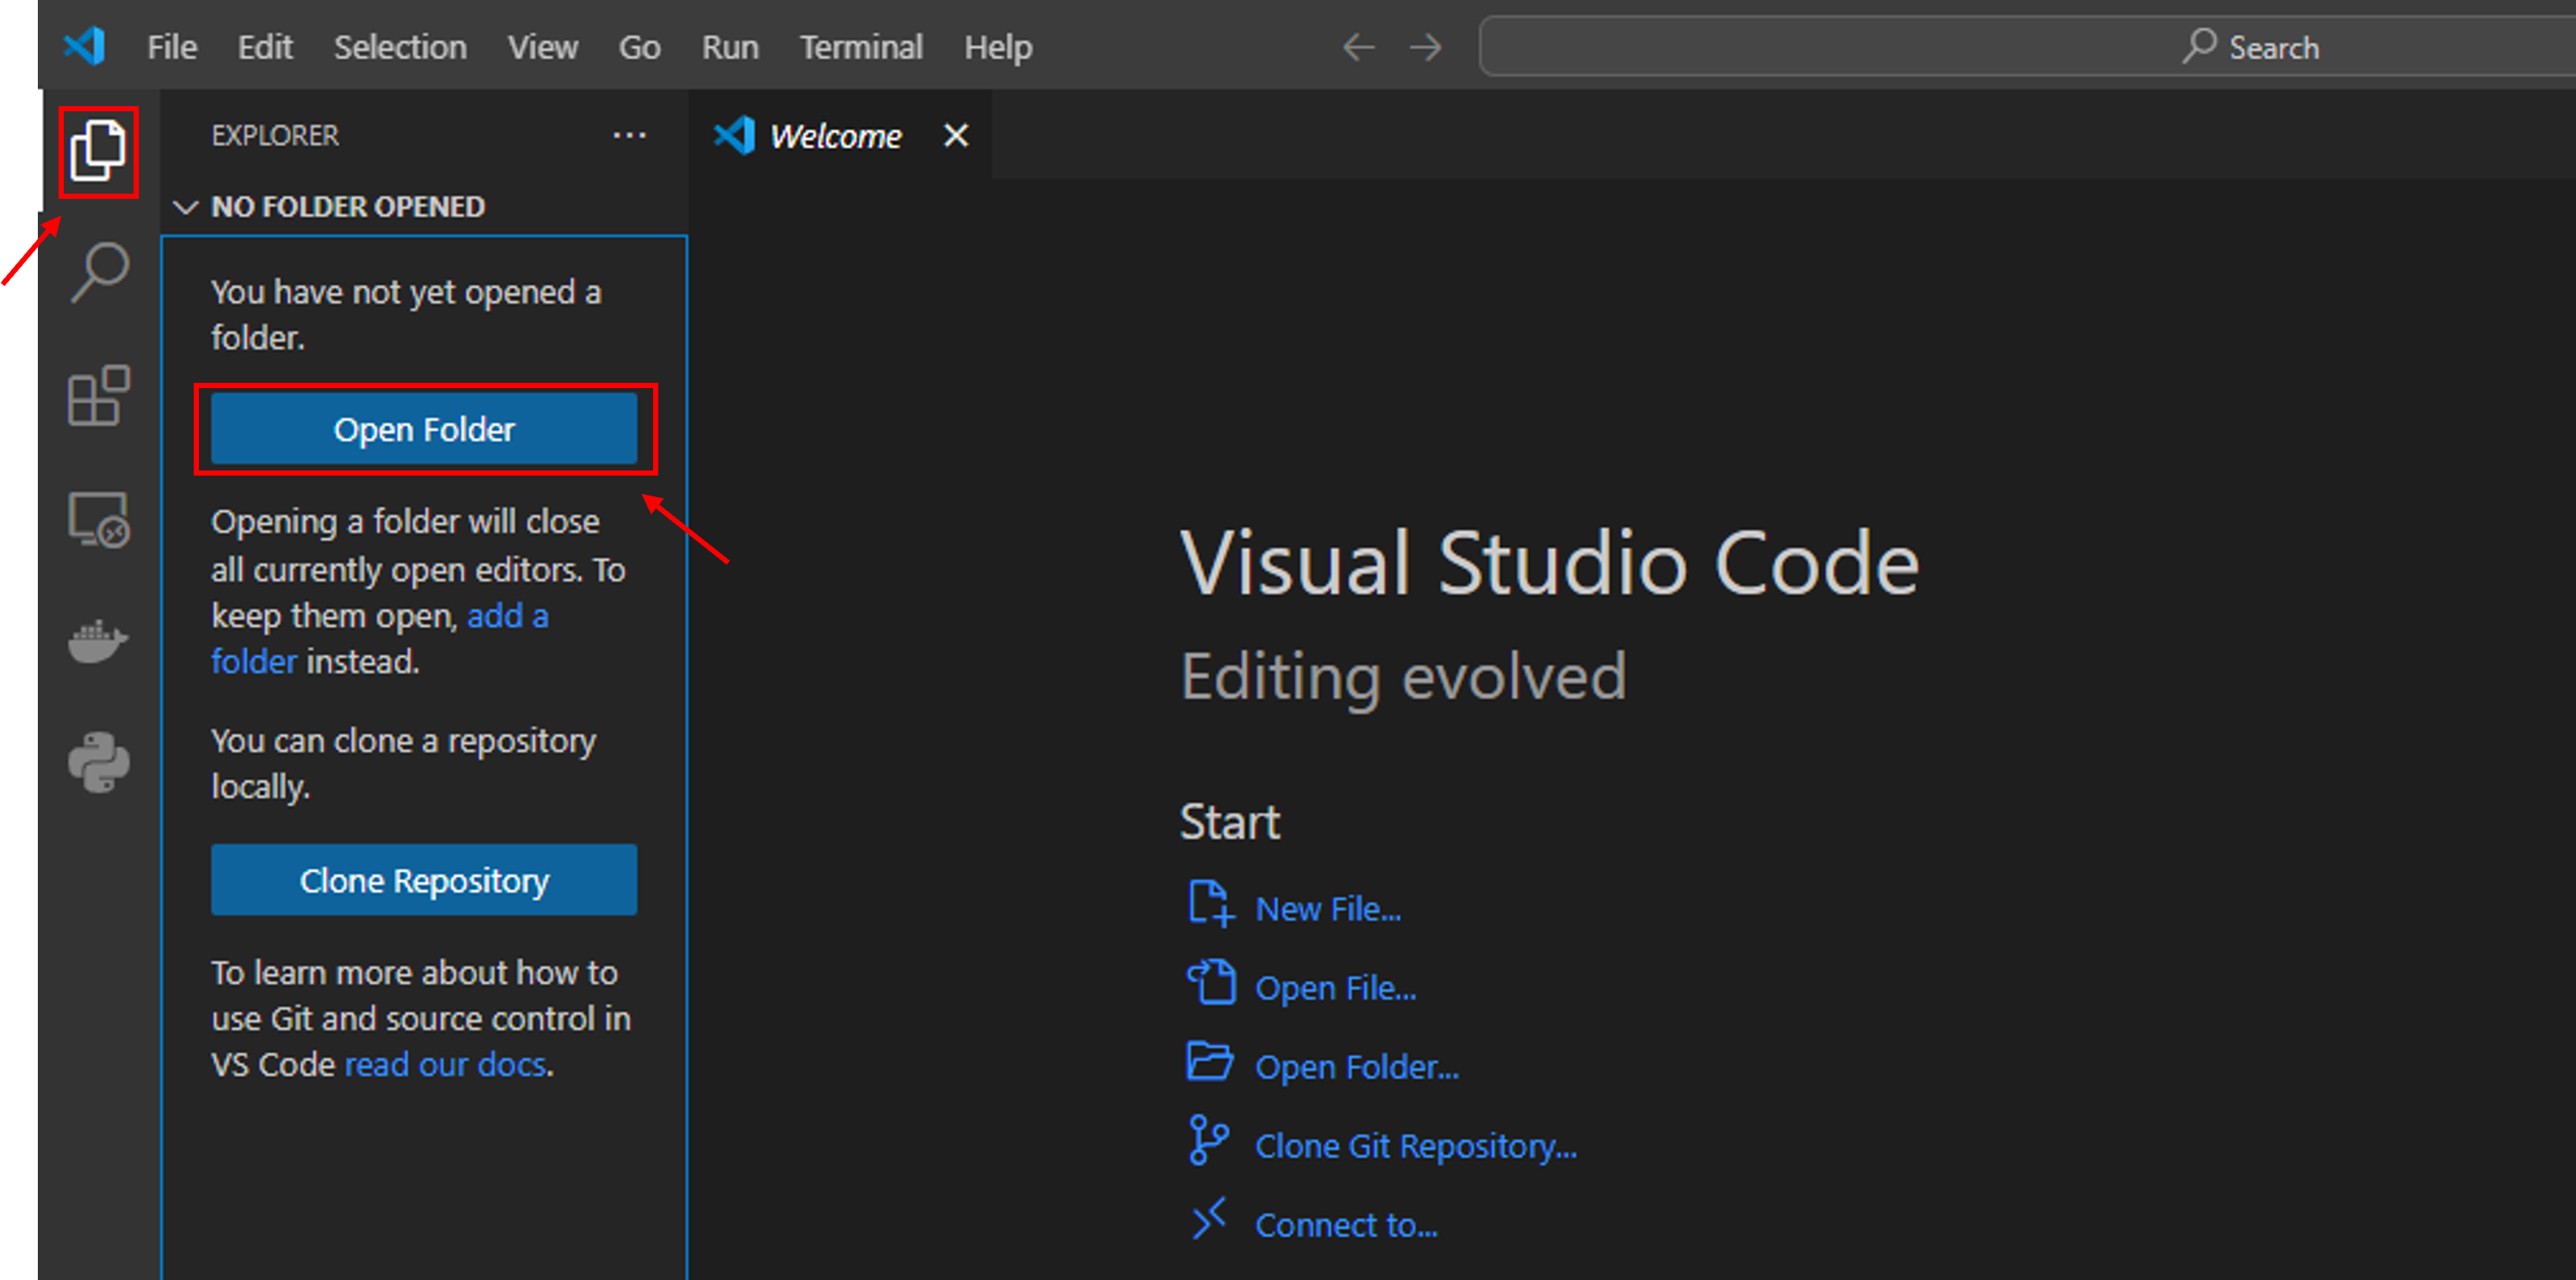
\includegraphics[width=0.85\textwidth]{images3/vscode-dir.png}
        \caption{Directorio de trabajo}
        \label{fig:semana3-vscode-dir}
    \end{subfigure}
    \begin{subfigure}{\textwidth}
        \centering
        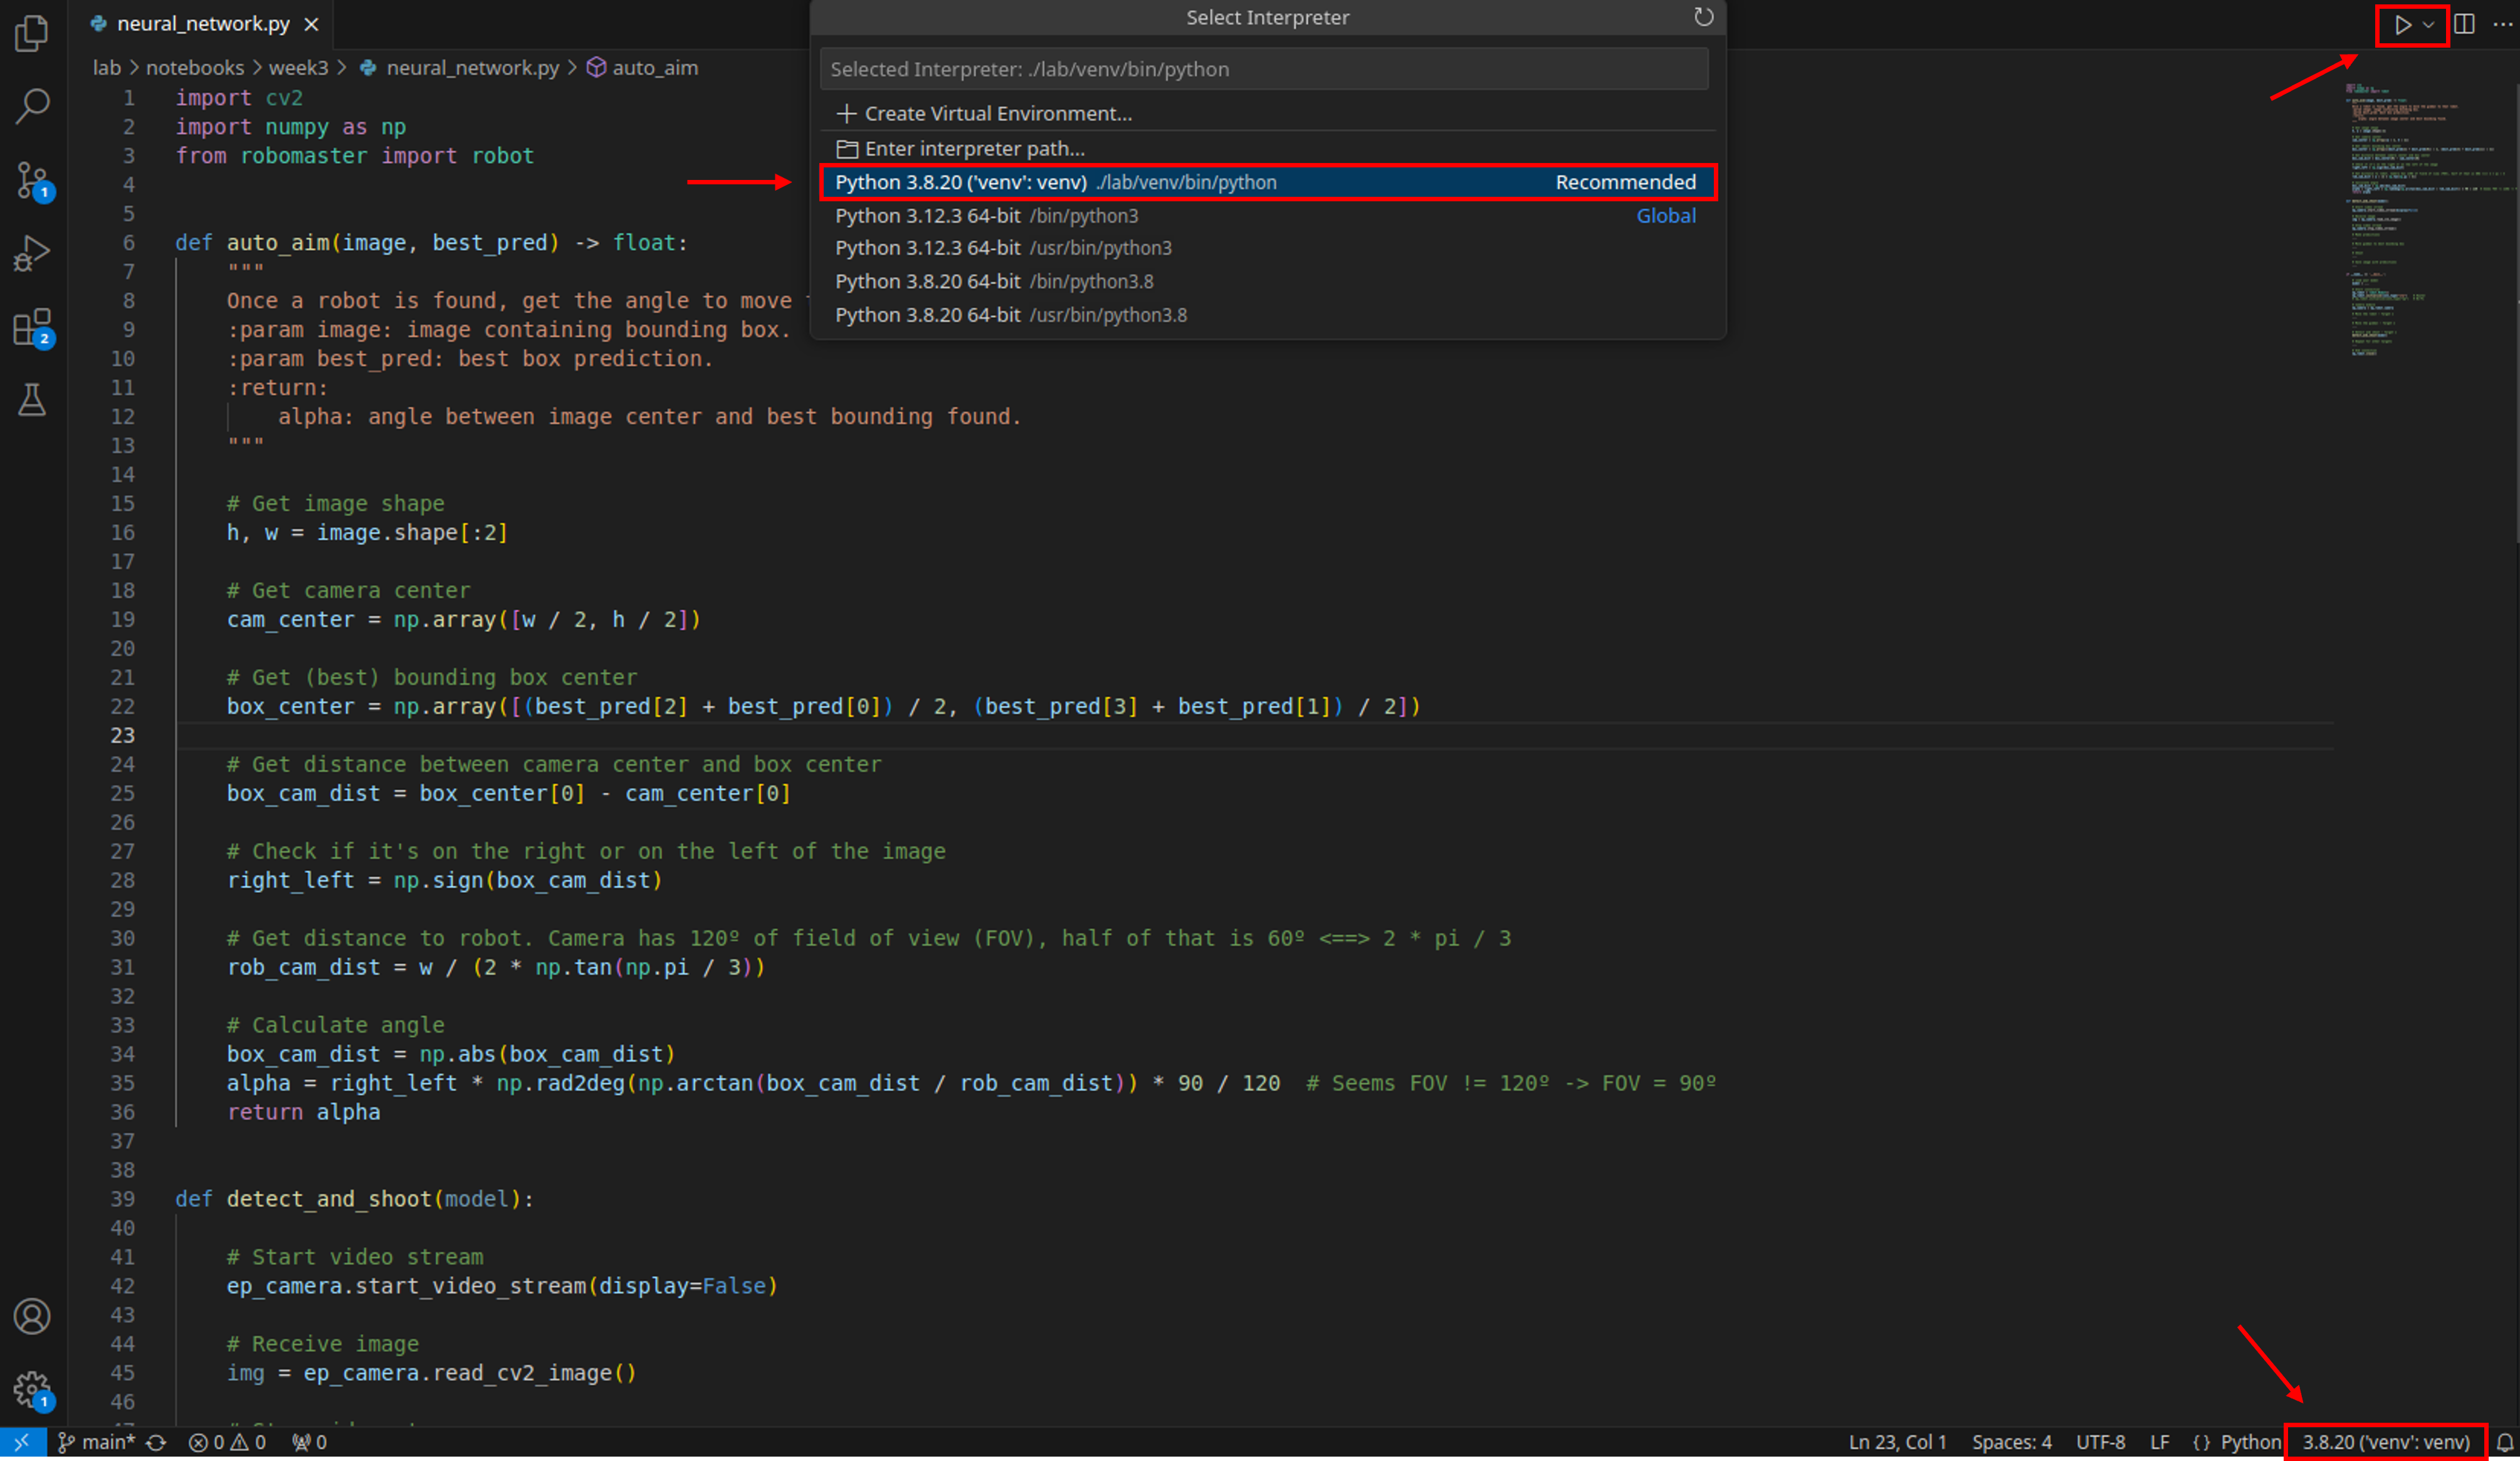
\includegraphics[width=0.8\textwidth]{images3/vscode-venv.png}
        \caption{Entorno virtual}
        \label{fig:semana3-vscode-venv}
    \end{subfigure}
    \caption{Configuración de VSCode.}
    \label{fig:semana3-vscode-config}
\end{figure}


% =============================================================================
\section{Uso del RoboMaster}
\label{sec:semana3-conexion}
% =============================================================================

Los RoboMasters admiten dos modos de conexión: ``Wi-Fi'' y ``networking''. El modo Wi-Fi es el que usamos en el Bloque 1: el robot emite su propia red. Como los ordenadores del laboratorio no tienen adaptador Wi-Fi, esta vez usaremos el modo networking, que consiste en mostrar al robot un código QR con los datos de la red del laboratorio para que se conecte a ella.

Abra \textit{connect.py}, escriba la SSID y la contraseña de la red del laboratorio y añada el número de serie de su RoboMaster (recuadro superior de la figura~\ref{fig:semana3-networking}). El número de serie no hace falta para conectarse, pero es la única forma de que su ordenador distinga su robot del de otro grupo conectado a la misma red. Sin él podría lanzar su script sobre el robot ajeno y provocar un accidente. El script lo guardará en \textit{serial\_number.txt}.

Antes de lanzarlo, prepare el robot (figura~\ref{fig:semana3-networking}): deslice la pestaña de conexión hasta el icono del router, que es el modo networking, y pulse el botón rojo que hay junto a ella para dejar al robot a la espera del código QR.

Lance entonces el script, agarre el robot y apunte con cuidado su cabeza hacia el QR emergente (si no aparece, abra el archivo \textit{qrcode.png}). El robot avisará cuando se haya conectado.


\begin{figure}[t]
    \centering
    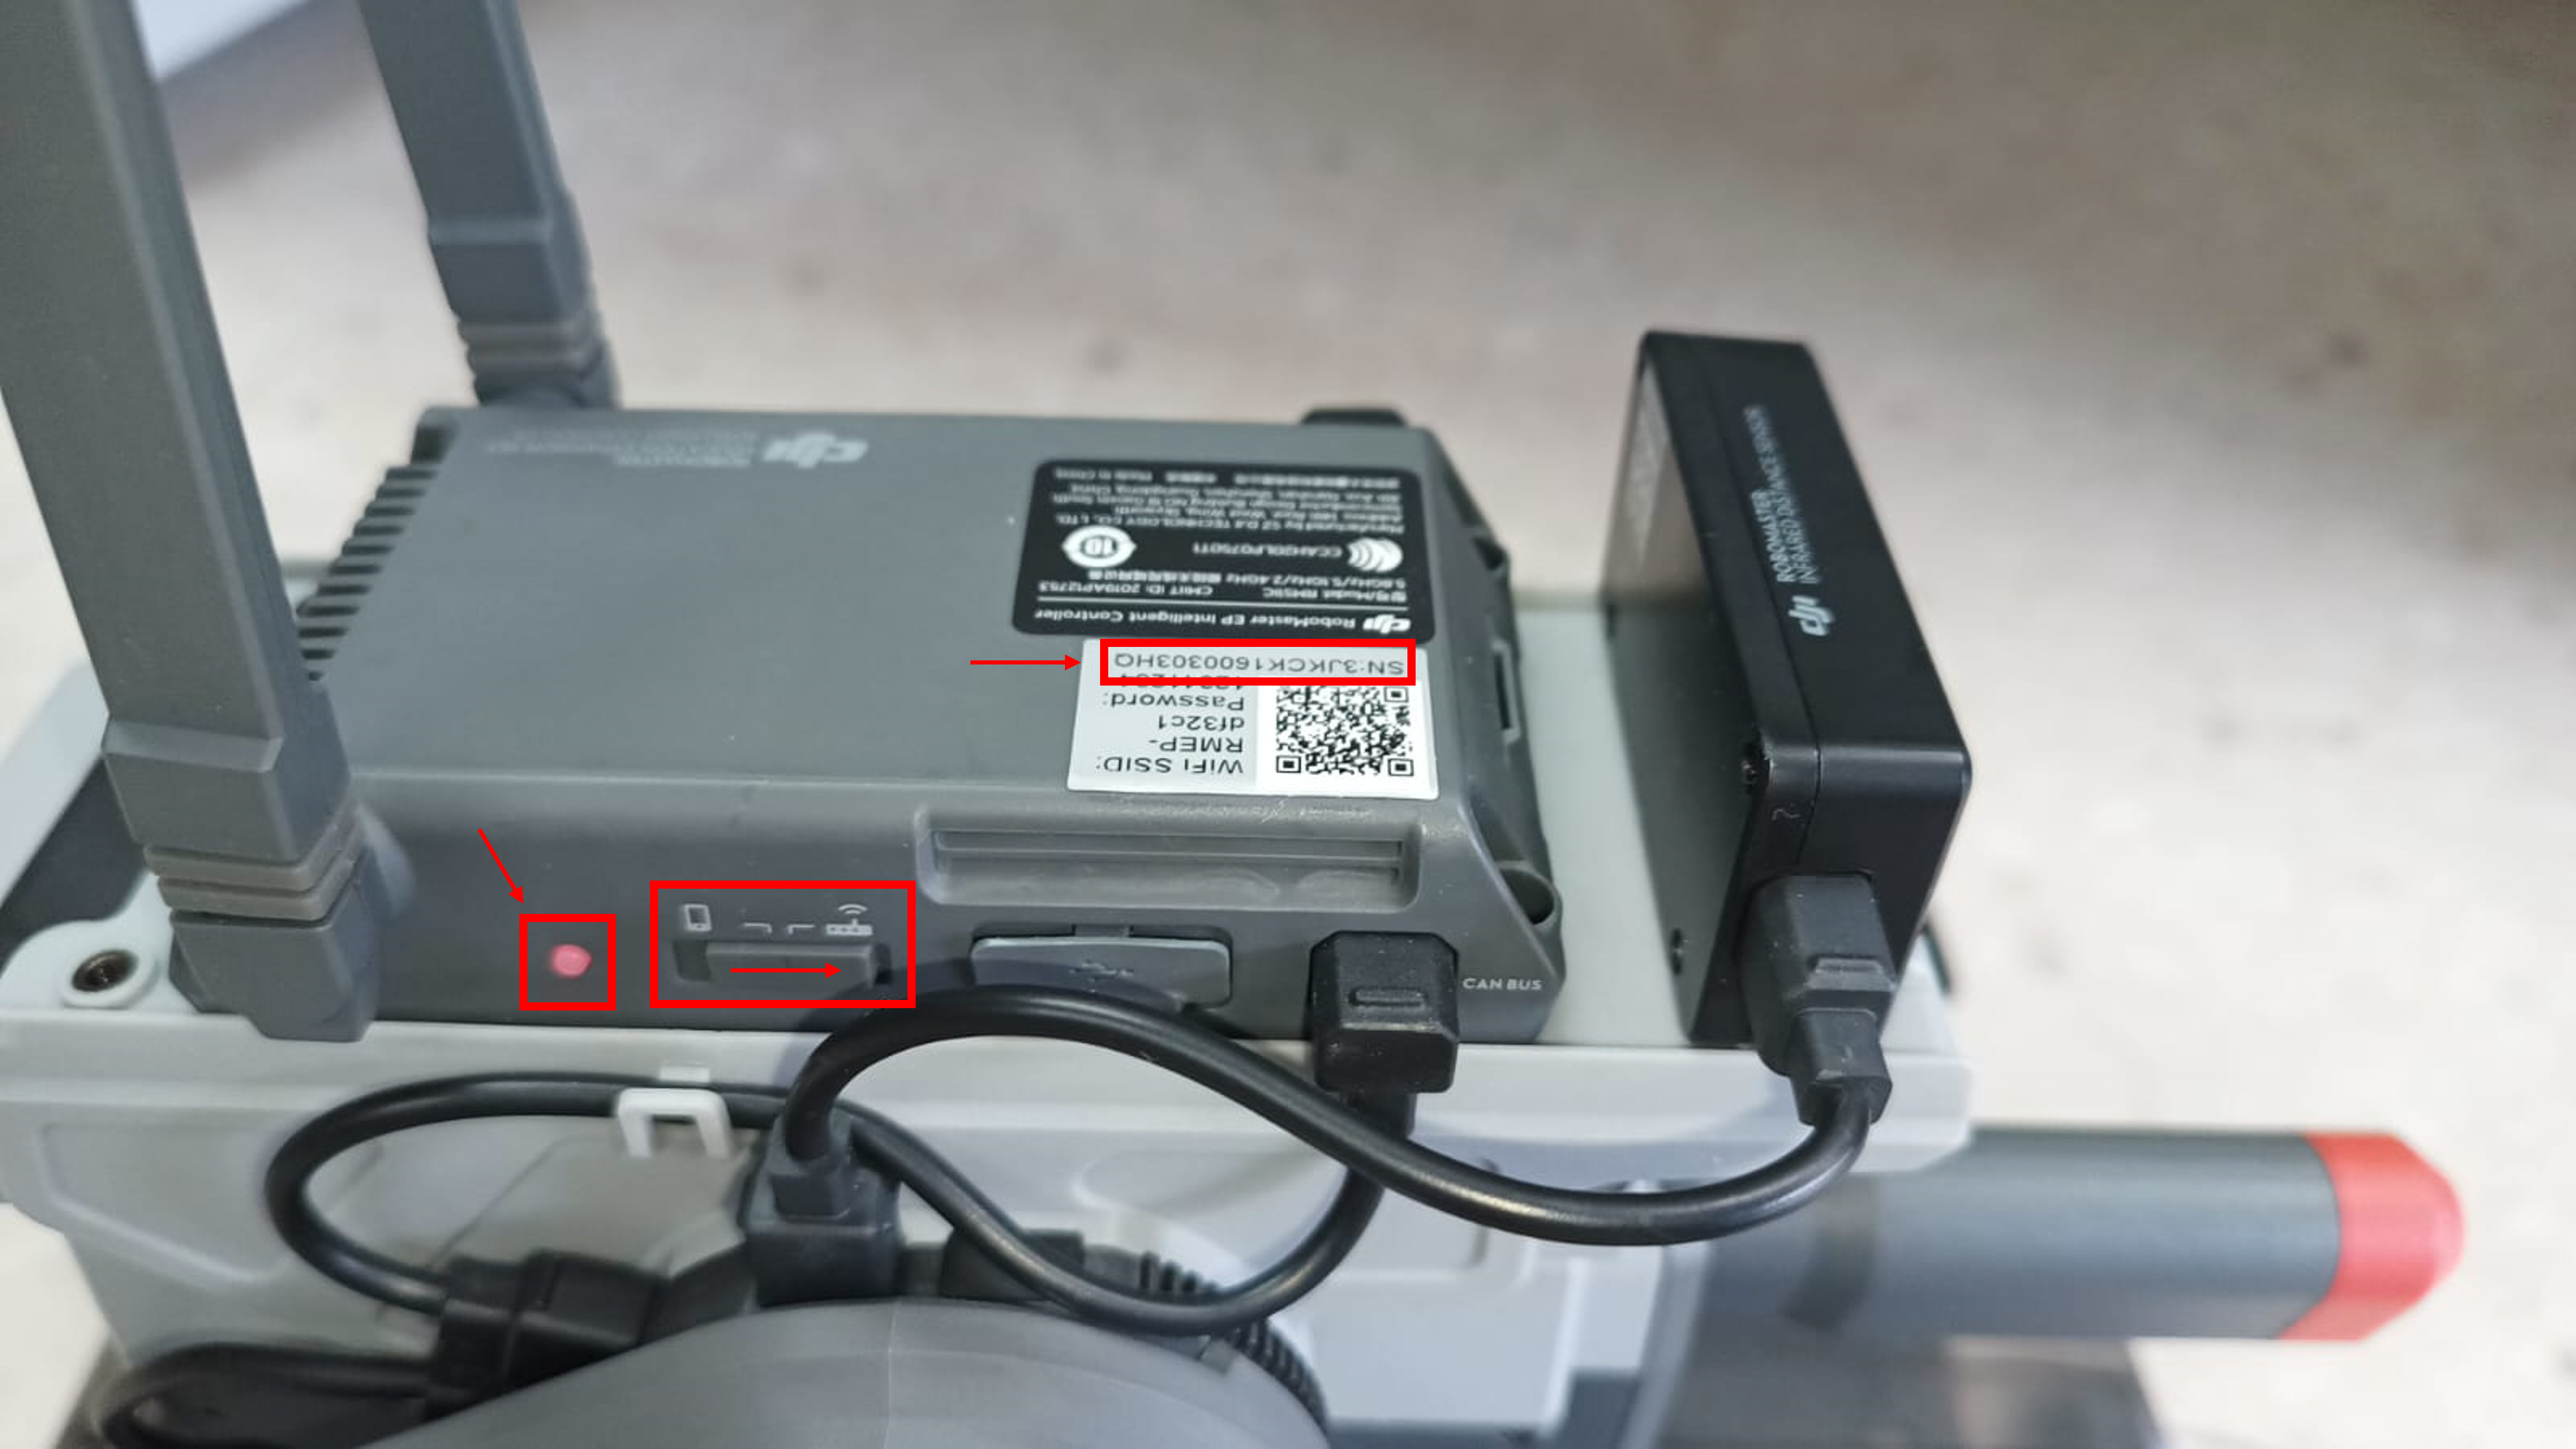
\includegraphics[width=0.7\textwidth]{images3/networking.png}
    \caption{Activar el modo ``networking'' para conectar el RoboMaster a la red Wi-Fi del laboratorio.}
    \label{fig:semana3-networking}
\end{figure}

% -----------------------------------------------------------------------------
\subsection{Módulos y scripts de ejemplo}
\label{sec:semana3-modulos}
% -----------------------------------------------------------------------------

El proyecto incluye uno o varios scripts de ejemplo por cada módulo del robot. Ejecútelos todos y analícelos con calma: son las piezas con las que construirá la demo, y \underline{en la demo final deberá usarlos todos}. Una vez los domine, podrá completar \textit{demo.py} y \textit{demo\_utils.py}, los scripts sobre los que programará el circuito final.


% =============================================================================
\section{El circuito}
\label{sec:semana3-circuito}
% =============================================================================

La evaluación final se hará sobre un circuito que pone a prueba todo lo desarrollado durante el proyecto. Constará de una serie de obstáculos que cada grupo deberá sortear (figura~\ref{fig:semana3-circuito}) y de puntos estratégicos desde los que buscar robots adversarios con la red del Bloque 2. Los objetivos detectados serán disparados con el blaster hasta inutilizarlos.

\begin{figure}[t]
    \centering
    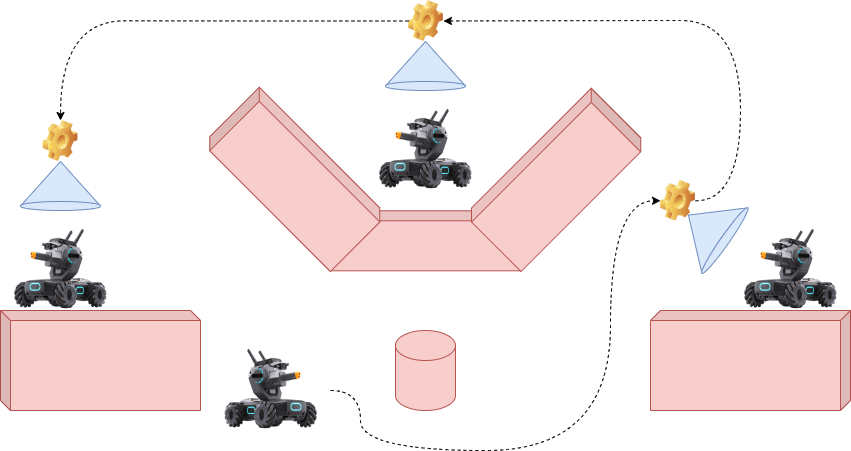
\includegraphics[width=0.8\textwidth]{images3/circuit.png}
    \caption{Circuito de ejemplo.}
    \label{fig:semana3-circuito}
\end{figure}

La estrategia de recorrido y de detección es la clave de esta semana. Detectar es costoso computacionalmente, así que no se trata de mirar todo el rato, sino de mirar donde y cuando conviene. Una estrategia habitual es la siguiente:

\begin{enumerate}
    \item \textbf{Desplazarse a un punto estratégico}, elegido por su visibilidad y por las posibles posiciones de los adversarios.
    \item \textbf{Detenerse y capturar una imagen} con la cámara.
    \item \textbf{Detectar} sobre esa imagen. Si no aparece ningún adversario, girar la torreta un ángulo fijo (por ejemplo, 90 grados), capturar de nuevo y repetir hasta completar un barrido de 360 grados (sin olvidarse después de resetear la posición de la cabeza).
    \item \textbf{Apuntar y disparar}: quedarse con las detecciones cuya confianza supere un umbral, usar la función de autoapuntado de \textit{demo.py} para calcular el ángulo y disparar con el blaster.
\end{enumerate}

Es solo un ejemplo. Cada grupo diseñará su propia estrategia, adaptándola a su circuito y a los recursos disponibles.


% =============================================================================
\section{Objetivos}
\label{sec:semana3-objetivos}
% =============================================================================

Hay libertad para diseñar el circuito, pero estos puntos son obligatorios:

\begin{itemize}
    \item \textbf{Recorrido:} dado un punto inicial y una serie de puntos de parada, diseñe un trayecto que pase por todos ellos \textbf{sin colisionar} con ningún obstáculo.
    \item \textbf{Objetivos:} inutilice a todos los RoboMasters del circuito (hacen falta 12 disparos por robot). Se entiende que el detector puede fallar en algún punto, sobre todo por la escasez de muestras de entrenamiento.
    \item \textbf{Estrategia de detección:} piense bien qué hacer en cada parada. ¿Disparar solo a la detección de mayor confianza o a todas las que superen el umbral? ¿Seguir girando la torreta hasta detectar algo o hasta completar los 360 grados?
    \item \textbf{Evidencias:} cada imagen sobre la que se aplique el detector debe guardarse en una carpeta dedicada, con las cajas predichas y su confianza dibujadas encima. Las necesitará para la memoria.
    \item \textbf{Módulos:} use \underline{obligatoriamente} todos los módulos del robot: chasis, torreta, cámara, blaster, LEDs y audio.
    \item \textbf{Originalidad:} se valoran los circuitos elaborados, los bailes, los obstáculos extra y, en general, cualquier añadido que mejore la demo.
\end{itemize}

\begin{framed}
    \textbf{NOTA}: trate a los robots con sumo cuidado. Está \textbf{PROHIBIDO} aumentar su velocidad. No confunda los ejes ``x'' e ``y'' (deje espacio en todas direcciones al hacer pruebas) y, cuando lance un script que mueva el robot, que un compañero lo siga de cerca para evitar colisiones; detenga el script de inmediato (Ctrl+C) ante cualquier riesgo. La torreta es delicada: no agarre nunca el robot por la cabeza, siempre por la base. Y no apunte a los ojos de nadie con el blaster.
\end{framed}

% -----------------------------------------------------------------------------
\subsection{Entregable}
\label{sec:semana3-entregable}
% -----------------------------------------------------------------------------

La memoria es \textbf{incremental}: esta es la última entrega y cierra el documento. Siga utilizando la plantilla \textit{PIDS-template.docx}. Para esta tercera entrega:

\begin{itemize}
    \item \textbf{Contenido:} los Bloques 1 y 2 corregidos y el Bloque 3 completo, que se cierra con las limitaciones del trabajo y las líneas de mejora. Rellene también la tabla ``Respuesta a la revisión anterior'': su ausencia penaliza la nota.
    \item \textbf{Extensión máxima:} 30 páginas de cuerpo, contando los Bloques 1 y 2. No cuentan la portada, el índice, la respuesta a la revisión anterior, el reparto del trabajo, las referencias ni los anexos.
    \item \textbf{Fichero:} un único PDF llamado \underline{\textbf{PIDS\_grupoX\_entregaN.pdf}}, donde X es el número de grupo y N el de la entrega. Por ejemplo, el grupo 3 entregaría \textit{PIDS\_grupo3\_entrega3.pdf}.
\end{itemize}

Se valorará el análisis honesto de la demo: una demostración imperfecta bien explicada puntúa más que una perfecta sin analizar correctamente.

\end{document}
